\chapter{动量能量习题课}
\section{作业习题}
\subsection*{一、填空题}

\begin{enumerate}
    \item 图中 \ref{fig:29} 沿着半径为$R$圆周运动的质点, 所受的几个力中有一个是恒力$\vec{F_0}$,方向始终沿$x$轴正向, 
    即, 当质点从$A$点沿逆时针方向走过$3/4$圆周到达$B$点时, 力$\vec{F_0}$所作的功为$A=\nl$.
    \begin{figure}[H]
        \centering
        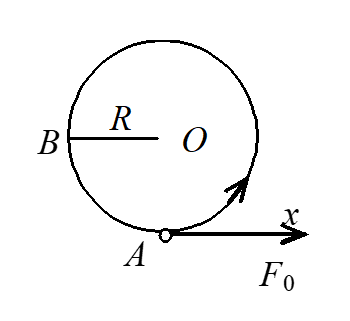
\includegraphics[width=0.15\textheight]{fig29}
            \caption{如图}\label{fig:29}
    \end{figure}
    \item 一个力$F$作用在质量为$2.0 kg$的质点上, 使之沿$x$轴运动. 已知在此力作用下质点的运动学方程
    为$x=3t-4t^2+t^3$(SI). 在0到$4s$的时间间隔内, 力$F$的冲量大小$I=\nl$.
    \item  质量为$m$的物体, 置于电梯内, 电梯以$g/3$加速度, 匀加速下降$h$,在此过程中, 
    电梯对物体的作用力所做的功$A=\nl$.
\end{enumerate}
\subsection*{二、选择题}
\begin{enumerate}
    \item 一水平放置的轻弹簧, 劲度系数为$k$, 其一端固定, 另一端系一质量为$m$的滑块$A$, 
    $A$旁又有一质量相同的滑块$B$, 如图所示\ref{fig:30}.设两滑块与桌面间无摩擦, 若用外力将$A$、$B$一起推压使弹簧压缩量为$d$而静止, 然后撤消外力, 则$B$离开时的速度为(\hspace{1pc})
    \fourch{$0$;}{$d\sqrt{\frac{k}{2m}}$ ;}{$d\sqrt{\frac{k}{m}}$;}{$d\sqrt{\frac{2k}{m}}$.}
    \begin{figure}[H]
        \centering
        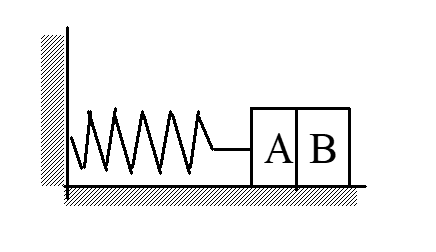
\includegraphics[width=0.15\textheight]{fig30}
            \caption{如图}\label{fig:30}
    \end{figure}
    \item 有一劲度系数为$k$的轻弹簧, 原长为$l_0$, 将它吊在天花板上. 当它下端挂一托盘平衡时, 其长度变为$l_1$. 然后在托盘中放一重物, 弹簧长度变为$l_2$, 则由$l_1$伸长至
    $l_2$的过程中, 弹性力所作的功为(\hspace{1pc})
    \fourch{$-\displaystyle{\int_{l_1}^{l_2}kx\mathrm{d}x}$;}{$\displaystyle{\int_{l_1}^{l_2}kx\mathrm{d}x}$;}
    {$\displaystyle{\int_{l_1-l_0}^{l_2-l_0}-kx\mathrm{d}x}$;}{$\displaystyle{\int_{l_1-l_0}^{l_2-l_0}kx\mathrm{d}x}$.}
    \item 质量分别为$m_1$、$m_2$的两个物体用一劲度系数为$k$的轻弹簧相联, 放在水平光滑桌面上. 当两物体相距$x$时, 系统由静止释放. 已知弹簧的自然长度为$x_0$, 则当物体相距$x_0$时, $m_1$的速度大小为(\hspace{1pc})
    \fourch{$\sqrt{\frac{k(x-x_0)^2}{m_1}}$;}{$\sqrt{\frac{k(x-x_0)^2}{m_2}}$;}{$\sqrt{\frac{k(x-x_0)^2}{m_1+m_2}}$;}{$\sqrt{\frac{k(x-x_0)^2}{m_1(m_1+m_2)}}$.}

\end{enumerate}
\subsection*{三、计算题}
\begin{enumerate}
    \item 如图 \ref{fig:31} ,用一弹簧把质量各为$m_1$和$m_2$的两木块连起来, 一起放在地面上, 弹簧的质量可不计, 而$m_2>m1$, 问:
    \begin{enumerate}
        \item[(1)] 对上面的木块必须施加多大的压力F, 以便在F突然撤去而上面的木块跳起来时, 恰能使下面的木块提离地面?
        \item[(2)] 如果$m_1$和$m_2$互换位置, 结果有无改变?
    \end{enumerate}
    \begin{figure}[H]
        \centering
        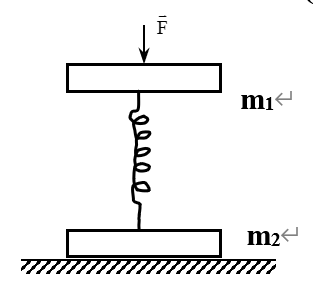
\includegraphics[width=0.15\textheight]{fig31}
            \caption{如图}\label{fig:31}
    \end{figure}
    \item 两个质量分别为$m_1$和$m_2$的木块$A$和$B$, 用一个质量忽略不计、劲度系数为$k$的弹簧联接起来, 放置在光滑水平面上, 使$A$紧靠墙壁, 如图所示\ref{fig:32}. 用力推木块$B$使弹簧压缩$x_0$,
    然后释放. 已知$m_1=m$, $m_2 = 3m$, 求:
    \begin{enumerate}
        \item[(1)] 释放后, 弹簧恢复到原长时$B$木块的速度为多大?
        \item[(2)] 释放后, $A$、$B$两木块速度相等时的瞬时速度的大小.
        \item[(3)] 释放后, 弹簧的最大伸长量.
    \end{enumerate}
    \begin{figure}[H]
        \centering
        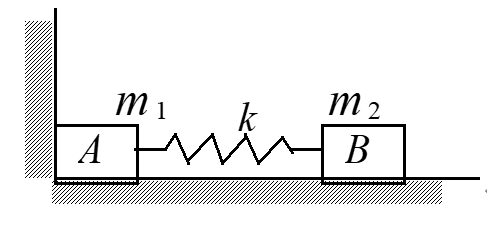
\includegraphics[width=0.15\textheight]{fig32}
            \caption{如图}\label{fig:32}
    \end{figure}
    \item 如图 \ref{fig:33}, 质量$m=0.1kg$的小球, 拴在长度$L=0.5m$的轻绳的一端, 构成摆, 摆动时与竖直的最大夹角为$60^\circ$. 求: 在$\theta<60^\circ$的任一位置, 求小球速度$V$与$\theta$的关系式, 
    这时小球的加速度为何? 绳的张力为多大?
    \begin{figure}[H]
        \centering
        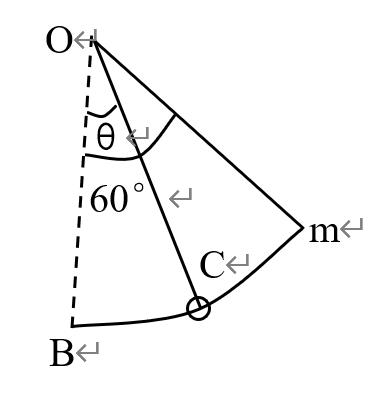
\includegraphics[width=0.13\textheight]{fig33}
            \caption{如图}\label{fig:33}
    \end{figure}
\end{enumerate}

\section{习题参考答案}
\subsection*{一、填空题}

\begin{enumerate}
    \item 图中 \ref{Fig:29} 沿着半径为$R$圆周运动的质点, 所受的几个力中有一个是恒力$\vec{F_0}$,方向始终沿$x$轴正向, 
    即, 当质点从$A$点沿逆时针方向走过$3/4$圆周到达$B$点时, 力$\vec{F_0}$所作的功为$A=\anl{$-F_0R$}$.
    \begin{figure}[H]
        \centering
        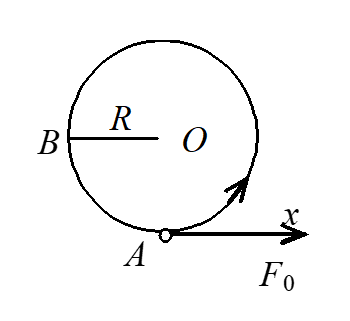
\includegraphics[width=0.15\textheight]{fig29}
            \caption{如图}\label{Fig:29}
    \end{figure}
    \begin{note}
        \textcolor{red}{$\mathrm{d}A=\vec{F}\cdot \mathrm{d}\vec{r}=F_0]mathrm{d}x$, $A = \displaystyle{\int_{0}^{-R}F_0\mathrm{d}x = -F_0R}$}
    \end{note}
    \item 一个力$F$作用在质量为$2.0 kg$的质点上, 使之沿$x$轴运动. 已知在此力作用下质点的运动学方程
    为$x=3t-4t^2+t^3$(SI). 在0到$4s$的时间间隔内, 力$F$的冲量大小$I=\anl{$32 N\cdot s$}$.
    \begin{note}
        \textcolor{red}{$V=\frac{\mathrm{d}x}{\mathrm{d}t=3-8t+3t^2}$ $\Longrightarrow$ $t=0$时, $V(0)=3$, $t=4$时, $V(4)=19$, $I=\Delta p = m\Delta V = 32 N\cdot s$}
    \end{note}
    \item  质量为$m$的物体, 置于电梯内, 电梯以$g/3$加速度, 匀加速下降$h$,在此过程中, 
    电梯对物体的作用力所做的功$A=\anl{$\frac{-2mgh}{3}$}$.
    \begin{note}
        看图, 懒得自己写了(其实自己写得不咋样):
    \end{note}
    \begin{figure}[H]
        \centering
        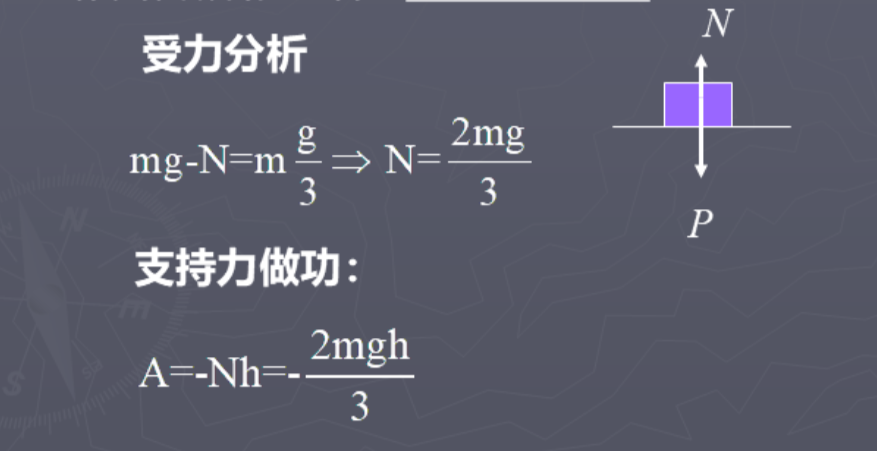
\includegraphics[width=0.25\textheight]{ans19}
    \end{figure}
\end{enumerate}

\subsection*{二、选择题}
\begin{enumerate}
    \item 一水平放置的轻弹簧, 劲度系数为$k$, 其一端固定, 另一端系一质量为$m$的滑块$A$, 
    $A$旁又有一质量相同的滑块$B$, 如图所示\ref{Fig:30}.设两滑块与桌面间无摩擦, 若用外力将$A$、$B$一起推压使弹簧压缩量为$d$而静止, 然后撤消外力, 则$B$离开时的速度为( B )
    \fourch{$0$;}{$d\sqrt{\frac{k}{2m}}$ ;}{$d\sqrt{\frac{k}{m}}$;}{$d\sqrt{\frac{2k}{m}}$.}
    \begin{figure}[h]
        \centering
        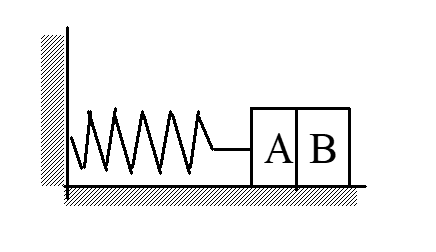
\includegraphics[width=0.15\textheight]{fig30}
            \caption{如图}\label{Fig:30}
    \end{figure}
    \begin{note}
        看图, 懒得自己写了(其实自己写得不咋样):
    \end{note}
    \begin{figure}[H]
        \centering
        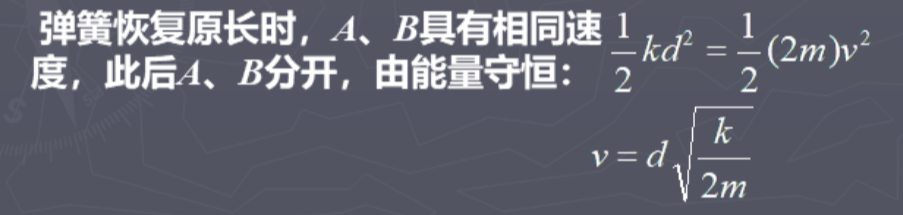
\includegraphics[width=0.25\textheight]{ans20}
    \end{figure}
    \item 有一劲度系数为$k$的轻弹簧, 原长为$l_0$, 将它吊在天花板上. 当它下端挂一托盘平衡时, 其长度变为$l_1$. 然后在托盘中放一重物, 弹簧长度变为$l_2$, 则由$l_1$伸长至
    $l_2$的过程中, 弹性力所作的功为( C )
    \fourch{$-\displaystyle{\int_{l_1}^{l_2}kx\mathrm{d}x}$;}{$\displaystyle{\int_{l_1}^{l_2}kx\mathrm{d}x}$;}
    {$\displaystyle{\int_{l_1-l_0}^{l_2-l_0}-kx\mathrm{d}x}$;}{$\displaystyle{\int_{l_1-l_0}^{l_2-l_0}kx\mathrm{d}x}$.}
    \begin{note}
        看图, 懒得自己写了(其实自己写得不咋样):
    \end{note}
    \begin{figure}[H]
        \centering
        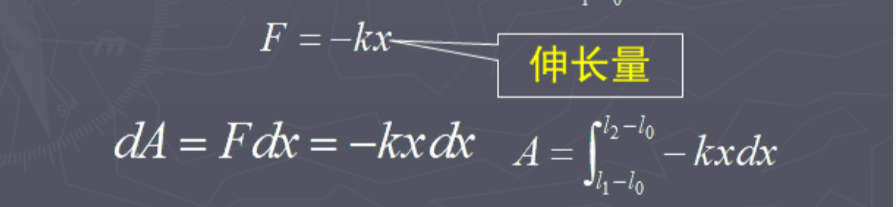
\includegraphics[width=0.25\textheight]{ans21}
    \end{figure}
    \item 质量分别为$m_1$、$m_2$的两个物体用一劲度系数为$k$的轻弹簧相联, 放在水平光滑桌面上. 当两物体相距$x$时, 系统由静止释放. 已知弹簧的自然长度为$x_0$, 则当物体相距$x_0$时, $m_1$的速度大小为( D )
    \fourch{$\sqrt{\frac{k(x-x_0)^2}{m_1}}$;}{$\sqrt{\frac{k(x-x_0)^2}{m_2}}$;}{$\sqrt{\frac{k(x-x_0)^2}{m_1+m_2}}$;}{$\sqrt{\frac{k(x-x_0)^2}{m_1(m_1+m_2)}}$.}
    \begin{note}
        \textcolor{red}{能量守恒: $\frac{1}{2}k(x-x_0)^2=\frac{1}{2}m_1V_1^2+\frac{1}{2}m_2V_2^2$}\\
        \textcolor{red}{动量守恒: $0=m_1V_1+m_2V_2$ 解出: $V_1=\sqrt{\frac{km_2(x-x_0)^2}{m_1(m_1+m_2)}}$}
    \end{note}
\end{enumerate}
\subsection*{三、计算题}
\begin{enumerate}
    \item 如图 \ref{Fig:31} ,用一弹簧把质量各为$m_1$和$m_2$的两木块连起来, 一起放在地面上, 弹簧的质量可不计, 而$m_2>m1$, 问:
    \begin{enumerate}
        \item[(1)] 对上面的木块必须施加多大的压力F, 以便在F突然撤去而上面的木块跳起来时, 恰能使下面的木块提离地面?
        \item[(2)] 如果$m_1$和$m_2$互换位置, 结果有无改变?
    \end{enumerate}
    \begin{figure}[H]
        \centering
        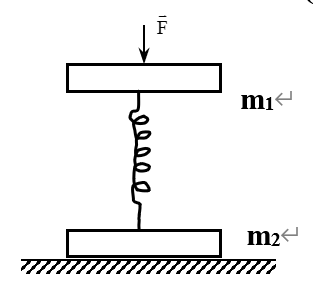
\includegraphics[width=0.15\textheight]{fig31}
            \caption{如图}\label{Fig:31}
    \end{figure}
    \begin{solution}
        看图: 
        \begin{figure}[H]
            \centering
            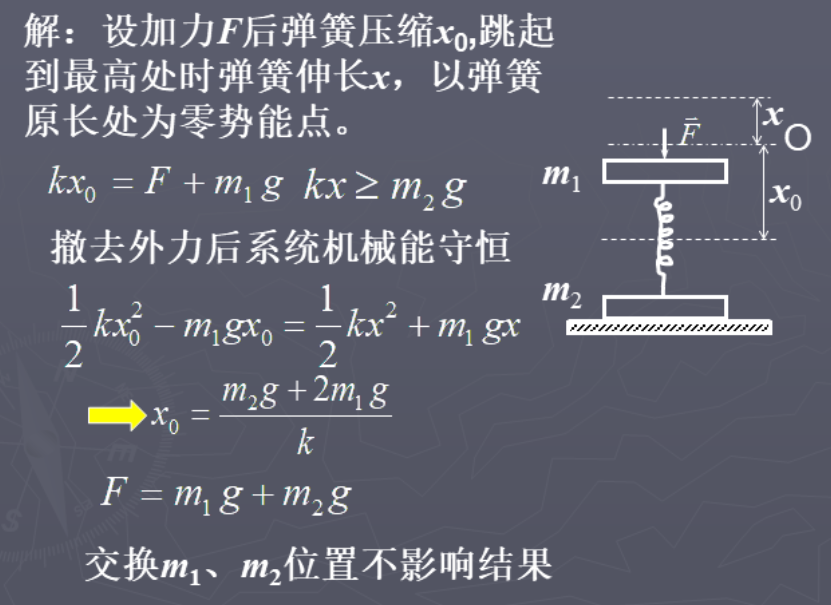
\includegraphics[width=0.48\textheight]{ans22}
        \end{figure}
    \end{solution}

    \item 两个质量分别为$m_1$和$m_2$的木块$A$和$B$, 用一个质量忽略不计、劲度系数为$k$的弹簧联接起来, 放置在光滑水平面上, 使$A$紧靠墙壁, 如图所示\ref{Fig:32}. 用力推木块$B$使弹簧压缩$x_0$,
    然后释放. 已知$m_1=m$, $m_2 = 3m$, 求:
    \begin{enumerate}
        \item[(1)] 释放后, 弹簧恢复到原长时$B$木块的速度为多大?
        \item[(2)] 释放后, $A$、$B$两木块速度相等时的瞬时速度的大小.
        \item[(3)] 释放后, 弹簧的最大伸长量.
    \end{enumerate}
    \begin{figure}[H]
        \centering
        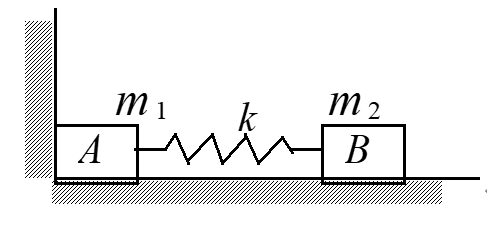
\includegraphics[width=0.15\textheight]{fig32}
            \caption{如图}\label{Fig:32}
    \end{figure}
    \begin{solution}
        \begin{enumerate}
            \item[(1)] 设弹簧恢复到原长时滑块$B$的速度为$V_{B0}$, 由机械能守恒得: $\frac{1}{2}kx_0^2=\frac{m_2V_{B0}^2}{2}$,\  $\therefore V_{B0}=x_0\sqrt{k/3m}$.
            \item[(2)]  $A$块离墙后: $m_1v_1+m_2v_2=m_2V_{B0}$, $v_1=v_2=v$时, $mv+3mv=3mV_{B0}$, $v=\frac{3}{4}V_{B0}=\frac{3}{4}x_0\sqrt{\frac{k}{3m}}$.
            \item[(3)] $\frac{1}{2}kx_0^2=\frac{(m_1+m_2)v^2}{2}+\frac{1}{2}kx^2$, \ \ $x=\frac{x_0}{2}$ 
        \end{enumerate}
    \end{solution}
    \item 如图 \ref{Fig:33}, 质量$m=0.1kg$的小球, 拴在长度$L=0.5m$的轻绳的一端, 构成摆, 摆动时与竖直的最大夹角为$60^\circ$. 求: 在$\theta<60^\circ$的任一位置, 求小球速度$V$与$\theta$的关系式, 
    这时小球的加速度为何? 绳的张力为多大?
    \begin{figure}[H]
        \centering
        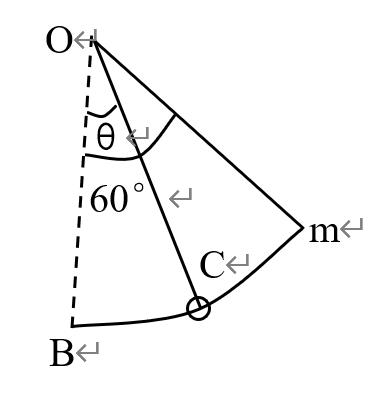
\includegraphics[width=0.13\textheight]{fig33}
            \caption{如图}\label{Fig:33}
    \end{figure}
    \begin{solution}
        摆动中机械能守恒: $-mgL\mathrm{cos}60^\circ = -mgL\mathrm{cos}\theta + \frac{mv^2}{2}$, $v=\sqrt{2gL(\mathrm{cos\theta-1/2})}$, $T-mg\mathrm{cos}\theta=ma_n=m\frac{v^2}{L}$, 带入$v$得
        $T=mg\mathrm{cos}\theta+2mg(\mathrm{cos}\theta-\frac{1}{2})=3mg\mathrm{cos}\theta-mg$.  $a_n=\frac{v^2}{L}=2g(\mathrm{cos}\theta-1/2)$, 
        $mg\mathrm{sin}\theta = ma_{\tau} \Longrightarrow a_{\tau} = g\mathrm{sin}\theta$, $\therefore \vec{a}=a_n\vec{n}+a_{\tau}\vec{\tau}$. $\vec{a}=2g(\mathrm{cos}\theta-1/2)\vec{n}+g\mathrm{sin}\vec{\tau}$.
    \end{solution}
\end{enumerate}